\documentclass[11pt]{article}
\usepackage[margin=1in]{geometry}
\usepackage{graphicx}
\usepackage{booktabs}
\usepackage{amsmath,amssymb}
\usepackage[T1]{fontenc}
\usepackage[colorlinks=true,linkcolor=blue,urlcolor=blue,citecolor=blue]{hyperref}
\usepackage{xcolor}
\IfFileExists{xurl.sty}{\usepackage{xurl}}{\usepackage{url}}
\setlength{\emergencystretch}{3em}
\setlength{\parskip}{0.35em}
\renewcommand{\arraystretch}{1.12}
% auto-generated: do not edit
\newcommand{\actDim}{8}
\newcommand{\actcleannFiveZeroEnsHi}{19.7}
\newcommand{\actcleannFiveZeroEnsLo}{9.0}
\newcommand{\actcleannFiveZeroEnsMean}{14.0}
\newcommand{\actcleannFiveZeroEnsSeedOne}{13}
\newcommand{\actcleannFiveZeroEnsSeedTwo}{14}
\newcommand{\actcleannFiveZeroEnsSeedZero}{15}
\newcommand{\actcleannFiveZeroEnsTerm}{1.3}
\newcommand{\actcleannFiveZeroEnsTwoHi}{20.3}
\newcommand{\actcleannFiveZeroEnsTwoLo}{8.3}
\newcommand{\actcleannFiveZeroRepHi}{25.0}
\newcommand{\actcleannFiveZeroRepLo}{13.0}
\newcommand{\actcleannFiveZeroRepMean}{18.7}
\newcommand{\actcleannFiveZeroRepSeedOne}{19}
\newcommand{\actcleannFiveZeroRepSeedTwo}{18}
\newcommand{\actcleannFiveZeroRepSeedZero}{19}
\newcommand{\actcleannFiveZeroRepTerm}{3.0}
\newcommand{\actcleannFiveZeroRepTwoHi}{25.7}
\newcommand{\actcleannFiveZeroRepTwoLo}{12.3}
\newcommand{\actcleannOneZeroZeroEnsHi}{31.0}
\newcommand{\actcleannOneZeroZeroEnsLo}{18.0}
\newcommand{\actcleannOneZeroZeroEnsMean}{24.3}
\newcommand{\actcleannOneZeroZeroEnsSeedOne}{19}
\newcommand{\actcleannOneZeroZeroEnsSeedTwo}{28}
\newcommand{\actcleannOneZeroZeroEnsSeedZero}{26}
\newcommand{\actcleannOneZeroZeroEnsTerm}{2.0}
\newcommand{\actcleannOneZeroZeroEnsTwoHi}{33.0}
\newcommand{\actcleannOneZeroZeroEnsTwoLo}{16.0}
\newcommand{\actcleannOneZeroZeroRepHi}{42.3}
\newcommand{\actcleannOneZeroZeroRepLo}{28.3}
\newcommand{\actcleannOneZeroZeroRepMean}{35.3}
\newcommand{\actcleannOneZeroZeroRepSeedOne}{36}
\newcommand{\actcleannOneZeroZeroRepSeedTwo}{35}
\newcommand{\actcleannOneZeroZeroRepSeedZero}{35}
\newcommand{\actcleannOneZeroZeroRepTerm}{4.0}
\newcommand{\actcleannOneZeroZeroRepTwoHi}{43.3}
\newcommand{\actcleannOneZeroZeroRepTwoLo}{27.3}
\newcommand{\actcleannTwoFiveEnsHi}{14.7}
\newcommand{\actcleannTwoFiveEnsLo}{7.0}
\newcommand{\actcleannTwoFiveEnsMean}{10.7}
\newcommand{\actcleannTwoFiveEnsSeedOne}{5}
\newcommand{\actcleannTwoFiveEnsSeedTwo}{16}
\newcommand{\actcleannTwoFiveEnsSeedZero}{11}
\newcommand{\actcleannTwoFiveEnsTerm}{0.7}
\newcommand{\actcleannTwoFiveEnsTwoHi}{18.0}
\newcommand{\actcleannTwoFiveEnsTwoLo}{4.3}
\newcommand{\actcleannTwoFiveRepHi}{13.0}
\newcommand{\actcleannTwoFiveRepLo}{5.3}
\newcommand{\actcleannTwoFiveRepMean}{9.0}
\newcommand{\actcleannTwoFiveRepSeedOne}{7}
\newcommand{\actcleannTwoFiveRepSeedTwo}{9}
\newcommand{\actcleannTwoFiveRepSeedZero}{11}
\newcommand{\actcleannTwoFiveRepTerm}{2.0}
\newcommand{\actcleannTwoFiveRepTwoHi}{14.3}
\newcommand{\actcleannTwoFiveRepTwoLo}{4.7}
\newcommand{\actnoiseOnenOneZeroZeroEnsHi}{0.0}
\newcommand{\actnoiseOnenOneZeroZeroEnsLo}{0.0}
\newcommand{\actnoiseOnenOneZeroZeroEnsMean}{0.0}
\newcommand{\actnoiseOnenOneZeroZeroEnsSeedOne}{0}
\newcommand{\actnoiseOnenOneZeroZeroEnsSeedTwo}{0}
\newcommand{\actnoiseOnenOneZeroZeroEnsSeedZero}{0}
\newcommand{\actnoiseOnenOneZeroZeroEnsTerm}{2.0}
\newcommand{\actnoiseOnenOneZeroZeroEnsTwoHi}{0.0}
\newcommand{\actnoiseOnenOneZeroZeroEnsTwoLo}{0.0}
\newcommand{\actnoiseOnenOneZeroZeroRepHi}{2.3}
\newcommand{\actnoiseOnenOneZeroZeroRepLo}{0.0}
\newcommand{\actnoiseOnenOneZeroZeroRepMean}{1.0}
\newcommand{\actnoiseOnenOneZeroZeroRepSeedOne}{1}
\newcommand{\actnoiseOnenOneZeroZeroRepSeedTwo}{1}
\newcommand{\actnoiseOnenOneZeroZeroRepSeedZero}{1}
\newcommand{\actnoiseOnenOneZeroZeroRepTerm}{2.7}
\newcommand{\actnoiseOnenOneZeroZeroRepTwoHi}{2.7}
\newcommand{\actnoiseOnenOneZeroZeroRepTwoLo}{0.0}
\newcommand{\actnoiseTwonOneZeroZeroEnsHi}{0.0}
\newcommand{\actnoiseTwonOneZeroZeroEnsLo}{0.0}
\newcommand{\actnoiseTwonOneZeroZeroEnsMean}{0.0}
\newcommand{\actnoiseTwonOneZeroZeroEnsSeedOne}{0}
\newcommand{\actnoiseTwonOneZeroZeroEnsSeedTwo}{0}
\newcommand{\actnoiseTwonOneZeroZeroEnsSeedZero}{0}
\newcommand{\actnoiseTwonOneZeroZeroEnsTerm}{1.3}
\newcommand{\actnoiseTwonOneZeroZeroEnsTwoHi}{0.0}
\newcommand{\actnoiseTwonOneZeroZeroEnsTwoLo}{0.0}
\newcommand{\actnoiseTwonOneZeroZeroRepHi}{0.0}
\newcommand{\actnoiseTwonOneZeroZeroRepLo}{0.0}
\newcommand{\actnoiseTwonOneZeroZeroRepMean}{0.0}
\newcommand{\actnoiseTwonOneZeroZeroRepSeedOne}{0}
\newcommand{\actnoiseTwonOneZeroZeroRepSeedTwo}{0}
\newcommand{\actnoiseTwonOneZeroZeroRepSeedZero}{0}
\newcommand{\actnoiseTwonOneZeroZeroRepTerm}{0.0}
\newcommand{\actnoiseTwonOneZeroZeroRepTwoHi}{0.0}
\newcommand{\actnoiseTwonOneZeroZeroRepTwoLo}{0.0}
\newcommand{\actnoiseZeroPtFivenOneZeroZeroEnsHi}{26.3}
\newcommand{\actnoiseZeroPtFivenOneZeroZeroEnsLo}{15.3}
\newcommand{\actnoiseZeroPtFivenOneZeroZeroEnsMean}{20.7}
\newcommand{\actnoiseZeroPtFivenOneZeroZeroEnsSeedOne}{25}
\newcommand{\actnoiseZeroPtFivenOneZeroZeroEnsSeedTwo}{18}
\newcommand{\actnoiseZeroPtFivenOneZeroZeroEnsSeedZero}{19}
\newcommand{\actnoiseZeroPtFivenOneZeroZeroEnsTerm}{3.7}
\newcommand{\actnoiseZeroPtFivenOneZeroZeroEnsTwoHi}{28.3}
\newcommand{\actnoiseZeroPtFivenOneZeroZeroEnsTwoLo}{13.7}
\newcommand{\actnoiseZeroPtFivenOneZeroZeroRepHi}{74.0}
\newcommand{\actnoiseZeroPtFivenOneZeroZeroRepLo}{59.7}
\newcommand{\actnoiseZeroPtFivenOneZeroZeroRepMean}{67.0}
\newcommand{\actnoiseZeroPtFivenOneZeroZeroRepSeedOne}{67}
\newcommand{\actnoiseZeroPtFivenOneZeroZeroRepSeedTwo}{64}
\newcommand{\actnoiseZeroPtFivenOneZeroZeroRepSeedZero}{70}
\newcommand{\actnoiseZeroPtFivenOneZeroZeroRepTerm}{1.3}
\newcommand{\actnoiseZeroPtFivenOneZeroZeroRepTwoHi}{75.3}
\newcommand{\actnoiseZeroPtFivenOneZeroZeroRepTwoLo}{58.3}
\newcommand{\batchSize}{128}
\newcommand{\chunkSize}{30}
\newcommand{\cmpActFlowEnsDelta}{+0.0}
\newcommand{\cmpActFlowEnsHi}{+8.7}
\newcommand{\cmpActFlowEnsLo}{-8.7}
\newcommand{\cmpActFlowEnsP}{=1}
\newcommand{\cmpActFlowEnsTwoHi}{+11.7}
\newcommand{\cmpActFlowEnsTwoLo}{-11.7}
\newcommand{\cmpActFlowRepDelta}{-21.3}
\newcommand{\cmpActFlowRepHi}{-14.0}
\newcommand{\cmpActFlowRepLo}{-29.0}
\newcommand{\cmpActFlowRepP}{<10^{-4}}
\newcommand{\cmpActFlowRepTwoHi}{-12.0}
\newcommand{\cmpActFlowRepTwoLo}{-30.7}
\newcommand{\cmpNoiseHalfEnsDelta}{-3.7}
\newcommand{\cmpNoiseHalfEnsHi}{+4.0}
\newcommand{\cmpNoiseHalfEnsLo}{-11.7}
\newcommand{\cmpNoiseHalfEnsP}{=0.41}
\newcommand{\cmpNoiseHalfEnsTwoHi}{+7.0}
\newcommand{\cmpNoiseHalfEnsTwoLo}{-14.3}
\newcommand{\cmpNoiseHalfRepDelta}{+31.7}
\newcommand{\cmpNoiseHalfRepHi}{+41.0}
\newcommand{\cmpNoiseHalfRepLo}{+22.0}
\newcommand{\cmpNoiseHalfRepP}{<10^{-4}}
\newcommand{\cmpNoiseHalfRepTwoHi}{+42.3}
\newcommand{\cmpNoiseHalfRepTwoLo}{+20.3}
\newcommand{\cmpNoiseOneEnsDelta}{-24.3}
\newcommand{\cmpNoiseOneEnsHi}{-18.0}
\newcommand{\cmpNoiseOneEnsLo}{-31.0}
\newcommand{\cmpNoiseOneEnsP}{<10^{-4}}
\newcommand{\cmpNoiseOneEnsTwoHi}{-16.0}
\newcommand{\cmpNoiseOneEnsTwoLo}{-33.0}
\newcommand{\cmpNoiseOneRepDelta}{-34.3}
\newcommand{\cmpNoiseOneRepHi}{-27.7}
\newcommand{\cmpNoiseOneRepLo}{-41.0}
\newcommand{\cmpNoiseOneRepP}{<10^{-4}}
\newcommand{\cmpNoiseOneRepTwoHi}{-26.7}
\newcommand{\cmpNoiseOneRepTwoLo}{-42.0}
\newcommand{\cmpNoiseTwoEnsDelta}{-24.3}
\newcommand{\cmpNoiseTwoEnsHi}{-18.0}
\newcommand{\cmpNoiseTwoEnsLo}{-31.0}
\newcommand{\cmpNoiseTwoEnsP}{<10^{-4}}
\newcommand{\cmpNoiseTwoEnsTwoHi}{-16.0}
\newcommand{\cmpNoiseTwoEnsTwoLo}{-33.0}
\newcommand{\cmpNoiseTwoRepDelta}{-35.3}
\newcommand{\cmpNoiseTwoRepHi}{-28.3}
\newcommand{\cmpNoiseTwoRepLo}{-42.3}
\newcommand{\cmpNoiseTwoRepP}{<10^{-4}}
\newcommand{\cmpNoiseTwoRepTwoHi}{-27.3}
\newcommand{\cmpNoiseTwoRepTwoLo}{-43.3}
\newcommand{\cmpQtyFiftyHundredEnsDelta}{+10.3}
\newcommand{\cmpQtyFiftyHundredEnsHi}{+16.7}
\newcommand{\cmpQtyFiftyHundredEnsLo}{+4.0}
\newcommand{\cmpQtyFiftyHundredEnsP}{=0.0024}
\newcommand{\cmpQtyFiftyHundredEnsTwoHi}{+19.0}
\newcommand{\cmpQtyFiftyHundredEnsTwoLo}{+1.3}
\newcommand{\cmpQtyFiftyHundredRepDelta}{+16.7}
\newcommand{\cmpQtyFiftyHundredRepHi}{+23.0}
\newcommand{\cmpQtyFiftyHundredRepLo}{+10.3}
\newcommand{\cmpQtyFiftyHundredRepP}{<10^{-4}}
\newcommand{\cmpQtyFiftyHundredRepTwoHi}{+24.7}
\newcommand{\cmpQtyFiftyHundredRepTwoLo}{+8.7}
\newcommand{\cmpQtyTwentyFiveFiftyEnsDelta}{+3.3}
\newcommand{\cmpQtyTwentyFiveFiftyEnsHi}{+8.3}
\newcommand{\cmpQtyTwentyFiveFiftyEnsLo}{-1.7}
\newcommand{\cmpQtyTwentyFiveFiftyEnsP}{=0.25}
\newcommand{\cmpQtyTwentyFiveFiftyEnsTwoHi}{+11.3}
\newcommand{\cmpQtyTwentyFiveFiftyEnsTwoLo}{-5.0}
\newcommand{\cmpQtyTwentyFiveFiftyRepDelta}{+9.7}
\newcommand{\cmpQtyTwentyFiveFiftyRepHi}{+15.7}
\newcommand{\cmpQtyTwentyFiveFiftyRepLo}{+4.0}
\newcommand{\cmpQtyTwentyFiveFiftyRepP}{=0.0022}
\newcommand{\cmpQtyTwentyFiveFiftyRepTwoHi}{+17.0}
\newcommand{\cmpQtyTwentyFiveFiftyRepTwoLo}{+2.7}
\newcommand{\cmpQtyTwentyFiveHundredEnsDelta}{+13.7}
\newcommand{\cmpQtyTwentyFiveHundredEnsHi}{+20.7}
\newcommand{\cmpQtyTwentyFiveHundredEnsLo}{+7.0}
\newcommand{\cmpQtyTwentyFiveHundredEnsP}{=1.8\times10^{-4}}
\newcommand{\cmpQtyTwentyFiveHundredEnsTwoHi}{+24.0}
\newcommand{\cmpQtyTwentyFiveHundredEnsTwoLo}{+3.0}
\newcommand{\cmpQtyTwentyFiveHundredRepDelta}{+26.3}
\newcommand{\cmpQtyTwentyFiveHundredRepHi}{+33.7}
\newcommand{\cmpQtyTwentyFiveHundredRepLo}{+19.0}
\newcommand{\cmpQtyTwentyFiveHundredRepP}{<10^{-4}}
\newcommand{\cmpQtyTwentyFiveHundredRepTwoHi}{+35.0}
\newcommand{\cmpQtyTwentyFiveHundredRepTwoLo}{+17.7}
\newcommand{\ctrlDt}{0.02}
\newcommand{\dataPoolOne}{0.4}
\newcommand{\dataPoolTwo}{0.0}
\newcommand{\dataPoolZero}{99.4}
\newcommand{\dataPoolZeroPtFive}{74.8}
\newcommand{\dataPoolZeroPtOne}{99.6}
\newcommand{\dataPoolZeroPtThree}{97.7}
\newcommand{\dataResetDev}{0}
\newcommand{\dataResidClean}{0.351}
\newcommand{\dataStepZeroDev}{1.24}
\newcommand{\dataSuccOne}{0}
\newcommand{\dataSuccTwo}{0}
\newcommand{\dataSuccZero}{100}
\newcommand{\dataSuccZeroPtFive}{71}
\newcommand{\dataSuccZeroPtOne}{99}
\newcommand{\dataSuccZeroPtThree}{97}
\newcommand{\dataTermOne}{13}
\newcommand{\dataTermTwo}{10}
\newcommand{\dataTermZero}{0}
\newcommand{\dataTermZeroPtFive}{7}
\newcommand{\dataTermZeroPtOne}{0}
\newcommand{\dataTermZeroPtThree}{0}
\newcommand{\dataTransOne}{14,093}
\newcommand{\dataTransTwo}{14,390}
\newcommand{\dataTransZero}{15,000}
\newcommand{\dataTransZeroPtFive}{14,636}
\newcommand{\dataTransZeroPtOne}{15,000}
\newcommand{\dataTransZeroPtThree}{15,000}
\newcommand{\diagEnsZOne}{22}
\newcommand{\diagEnsZTwo}{30}
\newcommand{\diagEnsZZero}{26}
\newcommand{\diagMaeRatioOne}{8.9}
\newcommand{\diagMaeRatioTwo}{8.9}
\newcommand{\diagMaeRatioZero}{9.0}
\newcommand{\diagMaeStudentOne}{0.651}
\newcommand{\diagMaeStudentTwo}{0.662}
\newcommand{\diagMaeStudentZero}{0.653}
\newcommand{\diagMaeTeacherOne}{0.073}
\newcommand{\diagMaeTeacherTwo}{0.075}
\newcommand{\diagMaeTeacherZero}{0.073}
\newcommand{\diagMaeTrainOne}{0.031}
\newcommand{\diagMaeTrainTwo}{0.032}
\newcommand{\diagMaeTrainZero}{0.031}
\newcommand{\diagOldestOne}{18}
\newcommand{\diagOldestTwo}{28}
\newcommand{\diagOldestZero}{26}
\newcommand{\diagTeacherFloor}{0.351}
\newcommand{\diagTestEnsOne}{21}
\newcommand{\diagTestEnsTwo}{28}
\newcommand{\diagTestEnsZero}{27}
\newcommand{\diagTestRepOne}{34}
\newcommand{\diagTestRepTwo}{31}
\newcommand{\diagTestRepZero}{35}
\newcommand{\diagTrainEnsOne}{32}
\newcommand{\diagTrainEnsTwo}{27}
\newcommand{\diagTrainEnsZero}{38}
\newcommand{\diagTrainRepOne}{35}
\newcommand{\diagTrainRepTwo}{33}
\newcommand{\diagTrainRepZero}{38}
\newcommand{\epLen}{150}
\newcommand{\evalSecMean}{54}
\newcommand{\flowcleannOneZeroZeroEnsHi}{31.3}
\newcommand{\flowcleannOneZeroZeroEnsLo}{17.7}
\newcommand{\flowcleannOneZeroZeroEnsMean}{24.3}
\newcommand{\flowcleannOneZeroZeroEnsSeedOne}{29}
\newcommand{\flowcleannOneZeroZeroEnsSeedTwo}{19}
\newcommand{\flowcleannOneZeroZeroEnsSeedZero}{25}
\newcommand{\flowcleannOneZeroZeroEnsTerm}{0.7}
\newcommand{\flowcleannOneZeroZeroEnsTwoHi}{33.3}
\newcommand{\flowcleannOneZeroZeroEnsTwoLo}{16.0}
\newcommand{\flowcleannOneZeroZeroRepHi}{19.0}
\newcommand{\flowcleannOneZeroZeroRepLo}{9.3}
\newcommand{\flowcleannOneZeroZeroRepMean}{14.0}
\newcommand{\flowcleannOneZeroZeroRepSeedOne}{14}
\newcommand{\flowcleannOneZeroZeroRepSeedTwo}{11}
\newcommand{\flowcleannOneZeroZeroRepSeedZero}{17}
\newcommand{\flowcleannOneZeroZeroRepTerm}{1.0}
\newcommand{\flowcleannOneZeroZeroRepTwoHi}{20.3}
\newcommand{\flowcleannOneZeroZeroRepTwoLo}{8.0}
\newcommand{\freshBase}{17777}
\newcommand{\freshDelta}{+47.0}
\newcommand{\freshFrozen}{2026-10-29}
\newcommand{\freshHi}{+54.7}
\newcommand{\freshLo}{+39.0}
\newcommand{\freshMcB}{48}
\newcommand{\freshMcC}{2}
\newcommand{\freshMcP}{<10^{-4}}
\newcommand{\freshNearest}{3.1}
\newcommand{\freshP}{<10^{-4}}
\newcommand{\freshSeedDeltaOne}{+47}
\newcommand{\freshSeedDeltaTwo}{+45}
\newcommand{\freshSeedDeltaZero}{+49}
\newcommand{\freshSha}{5e18af4383e3}
\newcommand{\freshTwoHi}{+56.0}
\newcommand{\freshTwoLo}{+37.7}
\newcommand{\freshVerdict}{confirmed}
\newcommand{\freshactcleannOneZeroZeroHi}{26.3}
\newcommand{\freshactcleannOneZeroZeroLo}{14.7}
\newcommand{\freshactcleannOneZeroZeroMean}{20.3}
\newcommand{\freshactcleannOneZeroZeroSeedOne}{20}
\newcommand{\freshactcleannOneZeroZeroSeedTwo}{20}
\newcommand{\freshactcleannOneZeroZeroSeedZero}{21}
\newcommand{\freshactcleannOneZeroZeroTwoHi}{27.3}
\newcommand{\freshactcleannOneZeroZeroTwoLo}{14.0}
\newcommand{\freshactnoiseZeroPtFivenOneZeroZeroHi}{74.7}
\newcommand{\freshactnoiseZeroPtFivenOneZeroZeroLo}{59.7}
\newcommand{\freshactnoiseZeroPtFivenOneZeroZeroMean}{67.3}
\newcommand{\freshactnoiseZeroPtFivenOneZeroZeroSeedOne}{67}
\newcommand{\freshactnoiseZeroPtFivenOneZeroZeroSeedTwo}{65}
\newcommand{\freshactnoiseZeroPtFivenOneZeroZeroSeedZero}{70}
\newcommand{\freshactnoiseZeroPtFivenOneZeroZeroTwoHi}{75.7}
\newcommand{\freshactnoiseZeroPtFivenOneZeroZeroTwoLo}{58.7}
\newcommand{\gpuName}{NVIDIA A100-SXM4-80GB}
\newcommand{\histLabelled}{13}
\newcommand{\histMislabelled}{14}
\newcommand{\histNever}{66}
\newcommand{\histReached}{18}
\newcommand{\histSucc}{27}
\newcommand{\hostName}{dcwipphhgc216}
\newcommand{\learnRate}{$10^{-4}$}
\newcommand{\menagerieSha}{1b86ece57659}
\newcommand{\modeactcleannFiveZeroDelta}{+4.7}
\newcommand{\modeactcleannFiveZeroHi}{+9.0}
\newcommand{\modeactcleannFiveZeroLo}{+0.3}
\newcommand{\modeactcleannOneZeroZeroDelta}{+11.0}
\newcommand{\modeactcleannOneZeroZeroHi}{+16.7}
\newcommand{\modeactcleannOneZeroZeroLo}{+5.3}
\newcommand{\modeactcleannTwoFiveDelta}{-1.7}
\newcommand{\modeactcleannTwoFiveHi}{+1.3}
\newcommand{\modeactcleannTwoFiveLo}{-4.7}
\newcommand{\modeactnoiseOnenOneZeroZeroDelta}{+1.0}
\newcommand{\modeactnoiseOnenOneZeroZeroHi}{+2.3}
\newcommand{\modeactnoiseOnenOneZeroZeroLo}{+0.0}
\newcommand{\modeactnoiseTwonOneZeroZeroDelta}{+0.0}
\newcommand{\modeactnoiseTwonOneZeroZeroHi}{+0.0}
\newcommand{\modeactnoiseTwonOneZeroZeroLo}{+0.0}
\newcommand{\modeactnoiseZeroPtFivenOneZeroZeroDelta}{+46.3}
\newcommand{\modeactnoiseZeroPtFivenOneZeroZeroHi}{+54.0}
\newcommand{\modeactnoiseZeroPtFivenOneZeroZeroLo}{+38.7}
\newcommand{\modeflowcleannOneZeroZeroDelta}{-10.3}
\newcommand{\modeflowcleannOneZeroZeroHi}{-3.0}
\newcommand{\modeflowcleannOneZeroZeroLo}{-17.7}
\newcommand{\nParamsAct}{12.7}
\newcommand{\nParamsFlow}{5.1}
\newcommand{\nVideos}{4}
\newcommand{\obsDim}{66}
\newcommand{\obsSimDev}{$1.2\times10^{-7}$}
\newcommand{\playgroundSha}{d59156e099a8}
\newcommand{\replayFirstBig}{27, 22, 36}
\newcommand{\replayResetDev}{0}
\newcommand{\tNewSuccOne}{0}
\newcommand{\tNewSuccTwo}{0}
\newcommand{\tNewSuccZero}{100}
\newcommand{\tNewSuccZeroPtFive}{65}
\newcommand{\tNewSuccZeroPtOne}{99}
\newcommand{\tNewSuccZeroPtThree}{97}
\newcommand{\tNewTermOne}{7}
\newcommand{\tNewTermTwo}{7}
\newcommand{\tNewTermZero}{0}
\newcommand{\tNewTermZeroPtFive}{10}
\newcommand{\tNewTermZeroPtOne}{0}
\newcommand{\tNewTermZeroPtThree}{0}
\newcommand{\tOldSuccOne}{1}
\newcommand{\tOldSuccTwo}{0}
\newcommand{\tOldSuccZero}{100}
\newcommand{\tOldSuccZeroPtFive}{70}
\newcommand{\tOldSuccZeroPtOne}{100}
\newcommand{\tOldSuccZeroPtThree}{98}
\newcommand{\taxactcleannOneZeroZeroEnsFail}{227}
\newcommand{\taxactcleannOneZeroZeroEnsLiftedFar}{28}
\newcommand{\taxactcleannOneZeroZeroEnsNoLift}{91}
\newcommand{\taxactcleannOneZeroZeroEnsNoTouch}{82}
\newcommand{\taxactcleannOneZeroZeroEnsShortHold}{20}
\newcommand{\taxactcleannOneZeroZeroEnsSucc}{73}
\newcommand{\taxactcleannOneZeroZeroEnsTerm}{6}
\newcommand{\taxactcleannOneZeroZeroRepFail}{194}
\newcommand{\taxactcleannOneZeroZeroRepLiftedFar}{46}
\newcommand{\taxactcleannOneZeroZeroRepNoLift}{77}
\newcommand{\taxactcleannOneZeroZeroRepNoTouch}{50}
\newcommand{\taxactcleannOneZeroZeroRepShortHold}{9}
\newcommand{\taxactcleannOneZeroZeroRepSucc}{106}
\newcommand{\taxactcleannOneZeroZeroRepTerm}{12}
\newcommand{\taxactnoiseZeroPtFivenOneZeroZeroEnsFail}{238}
\newcommand{\taxactnoiseZeroPtFivenOneZeroZeroEnsLiftedFar}{100}
\newcommand{\taxactnoiseZeroPtFivenOneZeroZeroEnsNoLift}{99}
\newcommand{\taxactnoiseZeroPtFivenOneZeroZeroEnsNoTouch}{11}
\newcommand{\taxactnoiseZeroPtFivenOneZeroZeroEnsShortHold}{17}
\newcommand{\taxactnoiseZeroPtFivenOneZeroZeroEnsSucc}{62}
\newcommand{\taxactnoiseZeroPtFivenOneZeroZeroEnsTerm}{11}
\newcommand{\taxactnoiseZeroPtFivenOneZeroZeroRepFail}{99}
\newcommand{\taxactnoiseZeroPtFivenOneZeroZeroRepLiftedFar}{50}
\newcommand{\taxactnoiseZeroPtFivenOneZeroZeroRepNoLift}{42}
\newcommand{\taxactnoiseZeroPtFivenOneZeroZeroRepNoTouch}{3}
\newcommand{\taxactnoiseZeroPtFivenOneZeroZeroRepShortHold}{1}
\newcommand{\taxactnoiseZeroPtFivenOneZeroZeroRepSucc}{201}
\newcommand{\taxactnoiseZeroPtFivenOneZeroZeroRepTerm}{3}
\newcommand{\teacherReloadDev}{0}
\newcommand{\teacherSteps}{60,000,000}
\newcommand{\teacherStepsReached}{63,897,600}
\newcommand{\teacherWallMin}{11}
\newcommand{\trainConcurrency}{eight}
\newcommand{\trainMinAct}{4.3}
\newcommand{\trainMinFlow}{1.5}
\newcommand{\trainSteps}{6,000}
\newcommand{\valContact}{100.0}
\newcommand{\valGripMaxMm}{29}
\newcommand{\valGripMedMm}{8}
\newcommand{\valLift}{100.0}
\newcommand{\valMinLiftCm}{20.6}
\newcommand{\valN}{814}
\newcommand{\valTwelve}{76}
\newcommand{\verbrax}{0.14.2}
\newcommand{\verflax}{0.11.2}
\newcommand{\verjax}{0.9.2}
\newcommand{\verjaxlib}{0.9.2}
\newcommand{\vermujoco}{3.15.0}
\newcommand{\vermujocomjx}{3.15.0}
\newcommand{\vernumpy}{2.5.4}
\newcommand{\verplayground}{0.2.0}
\newcommand{\verpython}{3.12.15}
\newcommand{\vertorch}{2.11.0+cu128}
\newcommand{\videoAgreeMax}{97}
\newcommand{\videoAgreeMin}{96}


\title{\textbf{CSCI 645 Homework 2}\\[2pt]
Imitation Learning for Robot Manipulation:\\
Demonstration Quantity and Quality for ACT on \texttt{PandaPickCube}}
\author{Yan Wen}
\date{Revised submission (protocol v2)}

\begin{document}
\maketitle
\vspace{-2.0em}

\begin{center}
\small
\begin{tabular}{ll}
\toprule
Environment & \texttt{PandaPickCube} (MuJoCo Playground), state-based, \texttt{impl=jax} \\
Teacher & PPO (Brax), \teacherSteps{} requested environment steps, seed 0 \\
Student & ACT, chunk $H=\chunkSize$; two inference modes (ensembling / replan every step) \\
Experiments & Option A (quantity 25/50/100) and Option B (teacher action noise $\sigma\in\{0.5,1,2\}$) \\
Models & 7 conditions $\times$ 3 training seeds $=$ 21 students \\
Evaluation & suite A: 100 held-out ICs; suite B: 100 fresh ICs, frozen protocol \\
Hardware & \gpuName{} (\hostName) \\
\bottomrule
\end{tabular}
\end{center}

\section*{Summary}
\textbf{What was run.} A PPO teacher on \texttt{PandaPickCube}; 100 clean
demonstrations (baseline) plus nested 25/50 subsets (Option A) and 100
demonstrations collected with teacher action noise $\sigma\in\{0.5,1,2\}$
(Option B); 21 ACT/flow-matching students; every student evaluated under two
inference modes on the same 100 held-out initial conditions (ICs; suite A), and
the moderate-noise comparison re-tested on 100 \emph{fresh} ICs under a protocol
frozen and pushed before any outcome existed (suite B).

\textbf{Findings.} (1) Baseline ACT (100 clean demos) succeeds
\actcleannOneZeroZeroEnsMean\% of the time with temporal ensembling and
\actcleannOneZeroZeroRepMean\% when replanning every step, against a teacher at
\tNewSuccZero\%. (2) More clean demonstrations help in both modes
($25\rightarrow100$: \cmpQtyTwentyFiveHundredEnsDelta{} and
\cmpQtyTwentyFiveHundredRepDelta{} percentage points). (3) Demonstrations from a
\emph{noisier} teacher ($\sigma=0.5$, teacher success \tOldSuccZeroPtFive\%) give a
much \emph{better} student when replanning (\actnoiseZeroPtFivenOneZeroZeroRepMean\%
vs \actcleannOneZeroZeroRepMean\%, \cmpNoiseHalfRepDelta\,pp), but not under
ensembling (\cmpNoiseHalfEnsDelta\,pp, CI includes 0); $\sigma\ge1$ destroys the
task. (4) The frozen fresh-IC test \textbf{\freshVerdict} the replanning result:
\freshactnoiseZeroPtFivenOneZeroZeroMean\% vs \freshactcleannOneZeroZeroMean\%
($\Delta=\freshDelta$\,pp, IC 95\% CI [\freshLo, \freshHi]). (5) The dominant
baseline failures are not reaching \emph{or} grasping alone: episodes split
between never touching the box, touching it without lifting it, and lifting it
without bringing it to the target.

\textbf{Corrections in this revision.} The termination-aware protocol changed
\emph{no} episode outcome in any of the 42 suite-A evaluations, so the original
headline numbers were not inflated by post-termination states. The original
failure analysis, however, was wrong: \histMislabelled{} of \histSucc{}
successful baseline episodes had received failure labels (mostly ``never reached
the box''), because the classifier tested the 12\,mm proximity before success.
All checkpoints were retrained (the originals were lost); retrained per-seed
results are close to the archived ones (Table~\ref{tab:oldnew}).

\begin{table}[t]
\centering
\scriptsize
\begin{adjustbox}{max width=\linewidth}
\begin{tabular}{lrrrrr}
\toprule
Condition & \#Demos & Teacher succ.\ (orig.) & Student, ensembling & Student, replan & Eval.\ episodes \\
\midrule
ACT, 25 clean & 25 & 100 (100) & 10.7 [7.0, 14.7] & 9.0 [5.3, 13.0] & 3 $\times$ 100 \\
ACT, 50 clean & 50 & 100 (100) & 14.0 [9.0, 19.7] & 18.7 [13.0, 25.0] & 3 $\times$ 100 \\
ACT, 100 clean (baseline) & 100 & 100 (100) & 24.3 [18.0, 31.0] & 35.3 [28.3, 42.3] & 3 $\times$ 100 \\
\midrule
ACT, 100 at $\sigma{=}0.5$ & 100 & 65 (70) & 20.7 [15.3, 26.3] & 67.0 [59.7, 74.0] & 3 $\times$ 100 \\
ACT, 100 at $\sigma{=}1$ & 100 & 0 (1) & 0.0 [0.0, 0.0] & 1.0 [0.0, 2.3] & 3 $\times$ 100 \\
ACT, 100 at $\sigma{=}2$ & 100 & 0 (0) & 0.0 [0.0, 0.0] & 0.0 [0.0, 0.0] & 3 $\times$ 100 \\
\midrule
Flow matching, 100 clean (suppl.) & 100 & 100 (100) & 24.3 [17.7, 31.3] & 14.0 [9.3, 19.0] & 3 $\times$ 100 \\
\bottomrule
\end{tabular}
\end{adjustbox}
\caption{The table required by Part 4 (success in \%, suite A, protocol v2). Teacher: the retrained teacher at the action-noise level of that condition's data on the same 100 ICs; in parentheses the original (data-collecting) teacher's archived v1 result. Student: mean of 3 training seeds with the IC-bootstrap 95\% CI; each seed is evaluated on the same 100 held-out ICs (300 episodes per condition, not 300 independent ICs).}
\label{tab:required}
\end{table}


\section{Task and demonstration source}
\textbf{Environment.} \texttt{PandaPickCube} from MuJoCo Playground: a Franka
Emika Panda must pick up a box and bring it to a target position sampled
$0.2$--$0.4$\,m \emph{above} the box's start (and within $\pm0.2$\,m in $x,y$),
so every success requires grasping and lifting. Observations are the
\obsDim-dimensional state vector of the environment's \texttt{\_get\_obs}: joint
positions (16) and velocities (15), gripper position (3) and orientation (6),
box orientation (6), box$-$gripper offset (3), target$-$box offset (3),
target$-$box orientation difference (6) and the control residual (8). Actions are
\actDim-dimensional joint-space deltas in $[-1,1]$, scaled by
\texttt{action\_scale}$=0.04$, added to the current control and clipped to the
actuator limits. Episodes last \epLen{} control steps of $\ctrlDt$\,s.

\textbf{Defining success.} The environment exposes no success signal: its
\texttt{done} flag fires only when the box leaves the workspace ($|x|,|y|,|z|>1$\,m
or $z<0$) or the physics state contains NaN, and \texttt{state.info} only carries
\texttt{reached\_box} (gripper site within 12\,mm of the box). We define:
\begin{quote}
an episode succeeds if the box is within 5\,cm of the target for 10 consecutive
\emph{valid} control steps (0.2\,s), measured from the simulator's box and target
positions.
\end{quote}
The hold stops a fly-through from counting. Reaching the hold once is a success
even if the box later leaves the radius; such later violations are reported
separately.

\textbf{Termination-aware evaluation (protocol v2).} The raw environment has no
auto-reset, so a batched rollout keeps stepping episodes whose box has already
left the workspace. The original submission (protocol v1) scored success over
the whole 150-step trace, including those post-termination states, and read the
distance from the observation. Protocol v2, used for every number in this
report, treats the first terminating transition's resulting state and all later
states as invalid: they are excluded from success, distances, returns (only the
terminating transition's own, finite, reward is counted) and every diagnostic;
non-finite states are never valid; a hold cannot span termination, an invalid
state or another episode. Unit tests cover normal success, an insufficient hold,
an apparent success that occurs only after termination, a valid success before a
later termination, NaN termination and cross-episode accumulation
(\texttt{tests/test\_metrics.py}). Per episode we save the reset keys, the valid
length and terminal cause, the distance traces and every diagnostic, so all
metrics can be recomputed without simulation. The observation-derived and
simulator box--target distances agree to \obsSimDev\,m on valid states.

\textbf{Teacher.} PPO from Brax with the hyperparameters MuJoCo Playground ships
for this task (\texttt{manipulation\_params.brax\_ppo\_config}: 2048 parallel
environments, learning rate $10^{-3}$, discount $0.97$, entropy cost $0.02$,
observation normalisation, policy MLP $4\times32$, value MLP $5\times256$),
trained for \teacherSteps{} requested environment steps (brax ran
\teacherStepsReached) instead of the shipped 20\,M, which was not enough for a
useful demonstrator in the original run. Demonstrations use the
\emph{deterministic} policy action.

\textbf{Provenance of the teacher and the data.} The demonstration datasets in
\texttt{data/} were collected by the \emph{original} teacher, whose checkpoint was
not recoverable. They are reused unchanged (SHA-256 recorded per model). The
teacher was \emph{retrained} with the same configuration and seed
(\teacherWallMin{} minutes on one GPU); the reloaded pickle reproduces the
in-memory policy (maximum action difference \teacherReloadDev). The retrained teacher is a new artifact,
\emph{not} the policy that generated the data: on the stored clean states its
action differs from the stored action by \dataResidClean{} on average
(per-dimension absolute difference; actions lie in $[-1,1]$). It is used only to
report teacher success under protocol v2 and as the reference in one diagnostic.
Table~\ref{tab:teacher} separates the original teacher's (archived) success, the
retrained teacher's success, and the success labels stored in the datasets. The
initial state of every stored episode matches a reset from its recorded
collection key (maximum difference \dataResetDev).

\begin{table}[t]
\centering
\scriptsize
%
\begin{tabular}{rrrrrrr}
\toprule
$\sigma$ & Orig.\ teacher & Retrained & Term.\,\% & Dataset succ. & Data term. & $|a_{\mathrm{data}}-a_{\mathrm{new}}|$ \\
\midrule
0 & 100 & 100/100 & 0 & 100/100 & 0 & 0.351 \\
0.1 & 100 & 99/100 & 0 & 99/100 & 0 & 0.337 \\
0.3 & 98 & 97/100 & 0 & 97/100 & 0 & 0.415 \\
0.5 & 70 & 65/100 & 10 & 71/100 & 7 & 0.516 \\
1 & 1 & 0/100 & 7 & 0/100 & 13 & 0.678 \\
2 & 0 & 0/100 & 7 & 0/100 & 10 & 0.809 \\
\bottomrule
\end{tabular}
%
\caption{Teacher provenance. `Orig.\ teacher': success (\%) of the ORIGINAL teacher that collected the datasets (archived, protocol v1). `Retrained': the retrained teacher on the same 100 held-out ICs (v2) and its share of terminated episodes. `Dataset succ.': stored success labels of the committed 100-episode datasets (identical under v2). `Data term.': dataset episodes truncated at termination. Last column: mean absolute difference between the stored actions and the retrained teacher's clipped action at the same states.}
\label{tab:teacher}
\end{table}


\textbf{Filtering.} The clean dataset keeps successful episodes only, but the
first 100 of the 512 collected all succeeded, so the filter removed nothing. The
noisy datasets keep the first 100 episodes \emph{including failures}, because
data quality is the independent variable. All stored success labels are
unchanged under protocol v2 (recomputed from the stored valid states; 0
disagreements in all six datasets).

\begin{figure}[t]
\centering
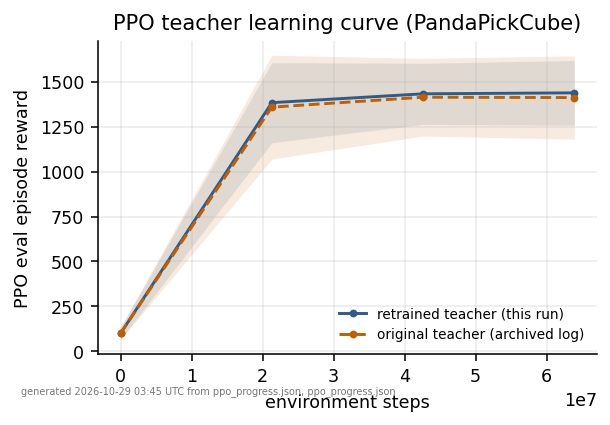
\includegraphics[width=0.62\linewidth]{figures/ppo_curve.png}
\caption{PPO teacher learning curves: the retrained teacher (this revision) and
the original teacher (archived log). Bands: across-episode standard deviation at
each evaluation point.}
\label{fig:ppo}
\end{figure}

\section{Demonstration quality}
\begin{table}[t]
\centering
\scriptsize
\begin{adjustbox}{max width=\linewidth}
\begin{tabular}{rrrrrrll}
\toprule
$\sigma$ & Eps. & Transitions & Mean len. & Term. & Succ. & Filter & Used by \\
\midrule
0 & 100 & 15,000 & 150.0 & 0 & 100 & success only & quantity + flow \\
0.1 & 100 & 15,000 & 150.0 & 0 & 99 & none & not used (preliminary) \\
0.3 & 100 & 15,000 & 150.0 & 0 & 97 & none & not used (preliminary) \\
0.5 & 100 & 14,636 & 146.4 & 7 & 71 & none & noise \\
1 & 100 & 14,093 & 140.9 & 13 & 0 & none & noise \\
2 & 100 & 14,390 & 143.9 & 10 & 0 & none & noise \\
\bottomrule
\end{tabular}
\end{adjustbox}
\caption{Committed demonstration datasets (collected by the original teacher). The clean set keeps successful episodes only (the first 100 of 512 collected all succeeded, so the filter removed none); noisy sets keep the first 100 episodes including failures. $\sigma{=}0.1, 0.3$ were a preliminary sweep that barely degraded the teacher and are not used by any student.}
\label{tab:data}
\end{table}

The baseline (clean) dataset has 100 episodes and \dataTransZero{} transitions;
every episode runs the full \epLen{} steps (the environment never terminates on
success) and all 100 succeed. The noisy datasets are shorter where the box was
knocked out of the workspace (\dataTermZeroPtFive, \dataTermOne{} and
\dataTermTwo{} episodes truncated at termination for $\sigma=0.5,1,2$) and contain
\dataSuccZeroPtFive, \dataSuccOne{} and \dataSuccTwo{} successful episodes.
Figure~\ref{fig:demos} shows box--target distance traces, coverage of initial
conditions and the executed-action distribution of the clean dataset; the
expert video is \texttt{videos/expert\_demo0\_success.mp4} and
Figure~\ref{fig:frames} shows frames.

\textbf{Observations.} The teacher is one deterministic policy, so trajectories
from nearby initial conditions are highly consistent and unimodal; the traces
show a reach phase, a lift that drives the distance down, and a hold. Initial box
and target positions cover the sampled square uniformly by construction (100
draws). One environment quirk matters for the analysis: the reset observation is
produced before MJX computes body positions, so in the first stored observation
of every episode the gripper and box positions read as zero (later
observations are correct; the student sees the same quirk at test time). Plots
and all position-based diagnostics therefore start at the first stepped state.
Visible inefficiencies: the approach to the box is often curved rather
than direct, and near the target the box keeps moving slightly instead of
settling, which is what the hold requirement measures.

\begin{figure}[t]
\centering
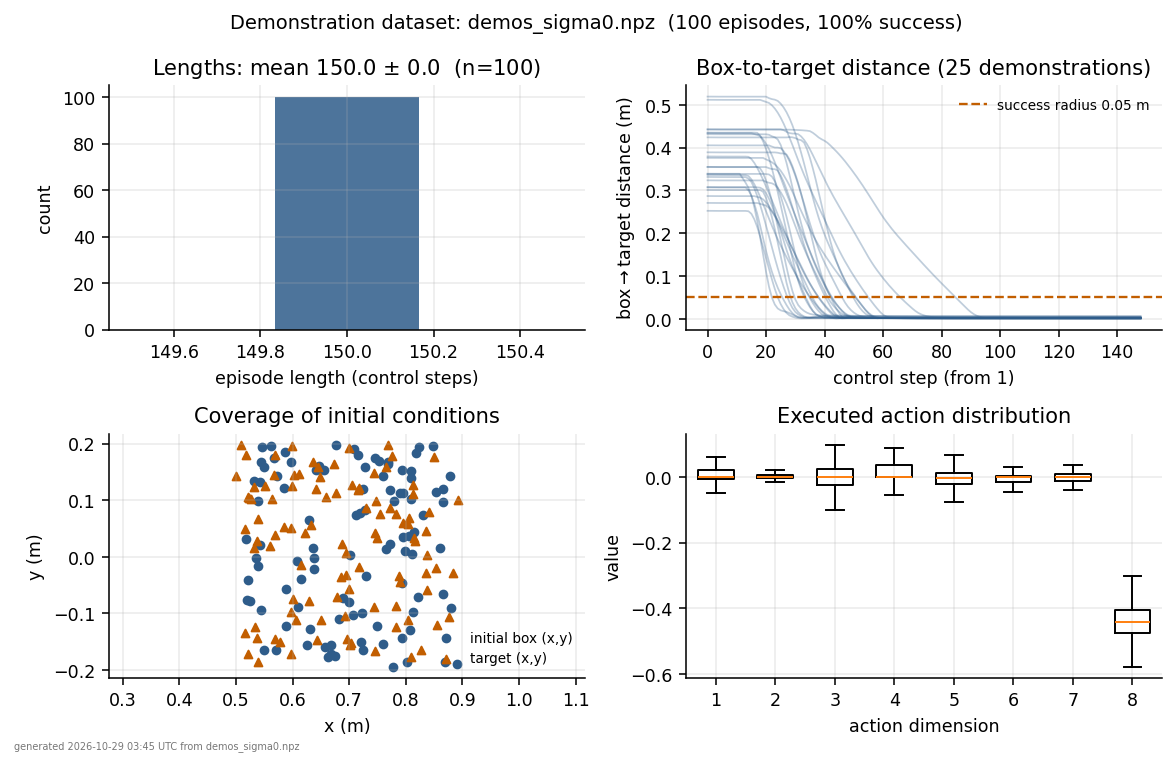
\includegraphics[width=\linewidth]{figures/demos.png}
\caption{Clean demonstration dataset: episode lengths, box--target distance
traces, initial box and target positions, and executed action distribution.}
\label{fig:demos}
\end{figure}

\section{Policy and training}
We use \textbf{ACT} (action chunking with transformers). Input: the standardised
\obsDim-dimensional state. Output: a chunk of $H=\chunkSize$ future actions
(\actDim{} each, i.e.\ 0.6\,s). Architecture: the transformer CVAE of the ACT
paper with hidden width 256, feed-forward width 1024, 8 heads, 4 encoder and 6
decoder layers, a 4-layer CVAE posterior encoder and a 32-dimensional latent
(\nParamsAct\,M parameters). The posterior encoder sees the observation and the
ground-truth chunk and emits $z$; the decoder maps $(z,\text{obs})$ through $H$
learned queries to the chunk. Objective: masked $L_1$ on the chunk plus
$10\cdot\mathrm{KL}$; at test time $z=0$. Chunks never cross an episode end
(padded steps are masked).

\textbf{Deviations from the reference implementation:} no image backbone (state
input, linear projection), pre-layer-norm GELU blocks, AdamW with warmup and
cosine decay, bf16 autocast, gradient clipping and an EMA of the weights, which
is what we evaluate. The code (\texttt{code/hw2/policies/act.py}) is a
re-implementation; nothing is vendored.

\textbf{Training.} \trainSteps{} steps, batch \batchSize, learning rate
\learnRate{} with 200 warmup steps and cosine decay to 5\%, weight decay
$10^{-4}$, AdamW $\beta=(0.9,0.95)$, gradient-norm clip 1, EMA decay 0.999.
Observations and actions are standardised per dimension with statistics fitted
on exactly the episodes each model trains on. Training seeds $\{0,1,2\}$ set
initialisation, data order and CVAE sampling. One ACT model took
\trainMinAct{} minutes on an A100 (eight models trained concurrently on four
GPUs); a flow-matching model \trainMinFlow{} minutes. Figure~\ref{fig:loss} shows
all 21 loss curves.

\textbf{Inference and action execution.} Predicted chunks are de-standardised and
clipped to $[-1,1]$. Two modes are evaluated for every model: \emph{temporal
ensembling} (the historical headline protocol: the policy is queried every step
and all chunk entries for the current step are averaged with weights
$\exp(-0.01\cdot\text{age})$, so the newest prediction weighs most; ACT's
reference weights the oldest most, which we evaluate as a diagnostic) and
\emph{replan every step} (a new chunk every step, only its first action executed).
Neither weighting, normalisation, clipping nor the success threshold was changed
relative to the original submission.

\begin{figure}[t]
\centering
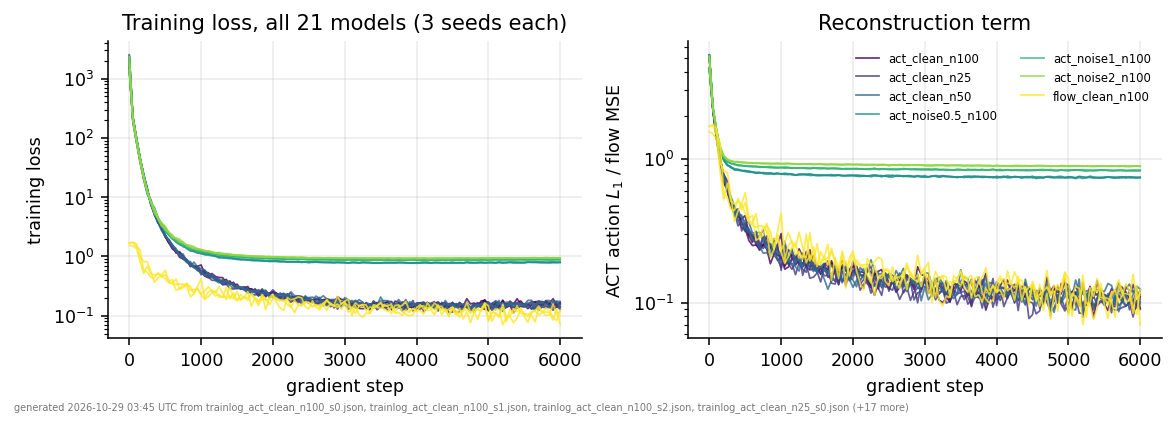
\includegraphics[width=\linewidth]{figures/loss.png}
\caption{Training loss of all 21 models (ACT: total loss and action $L_1$;
flow matching: velocity MSE).}
\label{fig:loss}
\end{figure}

\section{Baseline results}
\label{sec:baseline}
Table~\ref{tab:main} lists every model. The baseline (ACT, 100 clean
demonstrations) succeeds on \actcleannOneZeroZeroEnsMean\% of the 100 held-out ICs
with temporal ensembling (seeds \actcleannOneZeroZeroEnsSeedZero,
\actcleannOneZeroZeroEnsSeedOne, \actcleannOneZeroZeroEnsSeedTwo\%; IC 95\% CI
[\actcleannOneZeroZeroEnsLo, \actcleannOneZeroZeroEnsHi]) and
\actcleannOneZeroZeroRepMean\% when replanning every step (seeds
\actcleannOneZeroZeroRepSeedZero, \actcleannOneZeroZeroRepSeedOne,
\actcleannOneZeroZeroRepSeedTwo\%; [\actcleannOneZeroZeroRepLo,
\actcleannOneZeroZeroRepHi]). The retrained teacher succeeds on \tNewSuccZero/100
of the same ICs. The evaluation ICs (\texttt{split(PRNGKey(7777),100)}) are
disjoint from every demonstration-collection key; no training trajectory is
replayed. Rollout videos (verified as described in Section~\ref{sec:fail}):
\texttt{videos/student\_act\_clean\_n100\_s0\_replan1\_ep3\_success.mp4} and
\texttt{\dots\_ep8\_failure\_lifted-the-box-never-within-target-radius.mp4};
Figure~\ref{fig:frames} shows frames.

\textbf{Uncertainty.} Each condition has three trained models, and all of them
are evaluated on the same 100 ICs, so the 300 episodes are not 300 independent
trials: some ICs are hard for every seed. We therefore report the mean of the
three per-seed rates with two intervals: the \emph{IC interval} resamples ICs
with the trained models fixed (uncertainty about the IC distribution,
conditional on these models), and the \emph{2-way interval} also resamples
training seeds. With three seeds the latter is crude, and neither interval
describes the full distribution over training seeds; the per-seed values are
always shown. Contrasts between conditions are paired by IC; $p$-values are
sign-flip tests of the per-IC difference of seed-averaged success, conditional on
the models.

\textbf{Inference mode.} Replanning every step beats ensembling for the baseline
by \modeactcleannOneZeroZeroDelta\,pp (IC CI [\modeactcleannOneZeroZeroLo,
\modeactcleannOneZeroZeroHi]). Both modes were fixed in advance and are reported
for every model; ensembling remains the historical headline mode. Executing
chunks open loop is much worse (Table~\ref{tab:diag}).

\begin{table}[t]
\centering
\small
\begin{tabular}{llrrrrr}
\toprule
Condition & Algo. & \#Demos & $\sigma$ & Teacher succ. & Student succ. (95\% CI) & Eval. eps. \\
\midrule
Quantity & ACT & 25 & 0 & 100.0\% & 11.3\% [8.2, 15.4] & 300 \\
Quantity & ACT & 50 & 0 & 100.0\% & 14.7\% [11.1, 19.1] & 300 \\
Quantity & ACT & 100 & 0 & 100.0\% & 26.0\% [21.4, 31.2] & 300 \\
\midrule
Noisy teacher & ACT & 100 & 0.5 & 70.0\% & 20.7\% [16.5, 25.6] & 300 \\
Noisy teacher & ACT & 100 & 1 & 1.0\% & 0.0\% [0.0, 1.3] & 300 \\
Noisy teacher & ACT & 100 & 2 & 0.0\% & 0.0\% [0.0, 1.3] & 300 \\
\midrule
Flow matching & FLOW & 100 & 0 & 100.0\% & 22.0\% [17.7, 27.0] & 300 \\
\bottomrule
\end{tabular}
\caption{Teacher and student task success. Student success is pooled over all training seeds (3 seeds $\times$ 100 held-out initial conditions) with a Wilson 95\% interval. Teacher success is measured on the same held-out initial conditions, at the action-noise level used to collect that condition's data.}
\label{tab:main}
\end{table}


\begin{figure}[t]
\centering
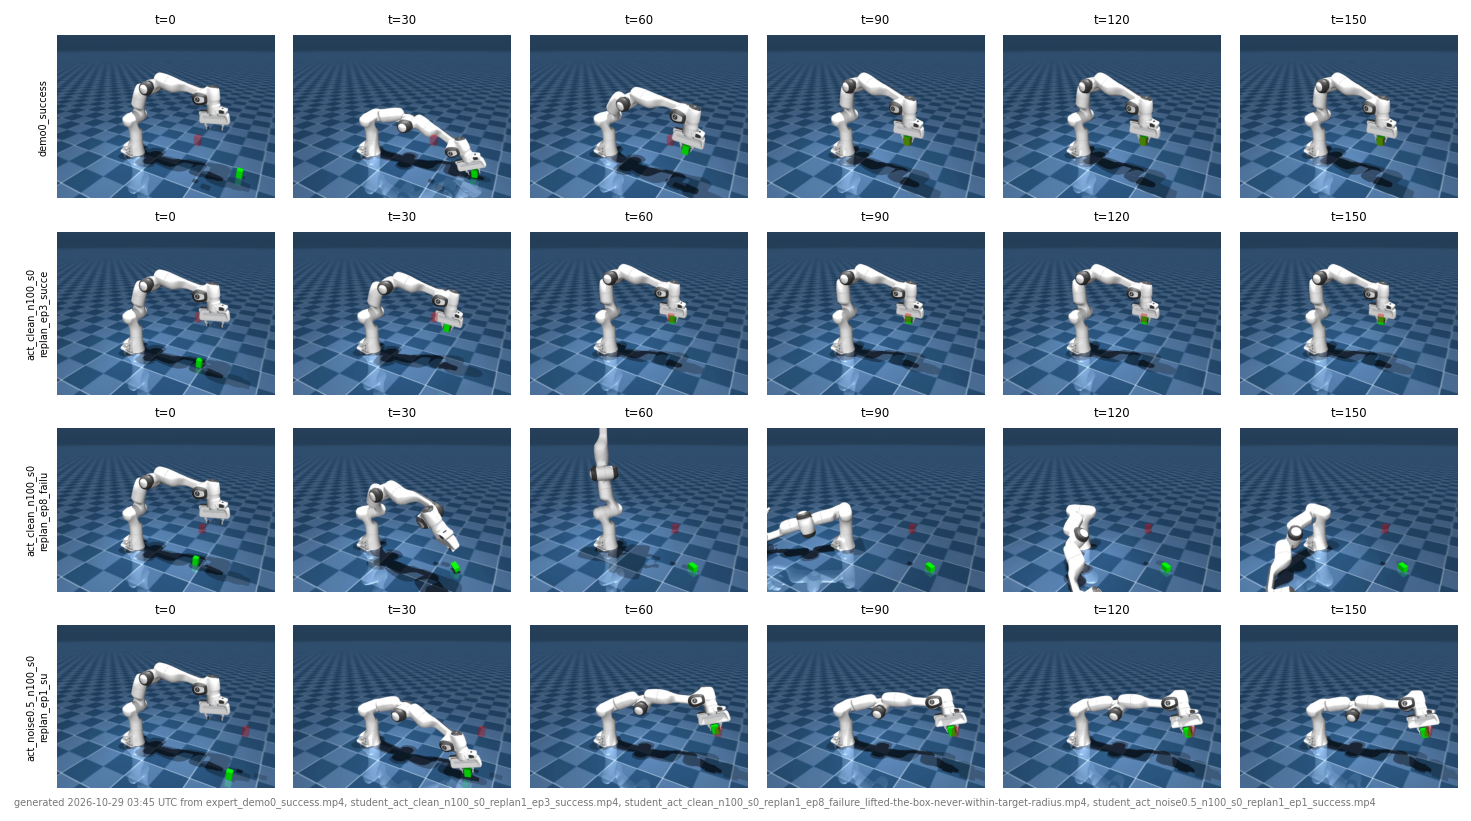
\includegraphics[width=\linewidth]{figures/frames.png}
\caption{Frames from the expert demonstration and the four verified student
clips (baseline and $\sigma=0.5$, seed 0, replanning; one success and one failure
each). Every 2nd control step is rendered; $t$ is the control step.}
\label{fig:frames}
\end{figure}

\section{Data ablation}
\textbf{Option A: quantity.} Students trained on nested prefixes (25 $\subset$ 50
$\subset$ 100) of the same clean dataset, with normalisation fitted on each
subset; nothing else changes. Success rises with quantity in both modes
(Figure~\ref{fig:quantity}, Table~\ref{tab:contrasts}): ensembling
\actcleannTwoFiveEnsMean{} $\rightarrow$ \actcleannFiveZeroEnsMean{} $\rightarrow$
\actcleannOneZeroZeroEnsMean\%, replanning \actcleannTwoFiveRepMean{}
$\rightarrow$ \actcleannFiveZeroRepMean{} $\rightarrow$
\actcleannOneZeroZeroRepMean\%. $25\rightarrow100$ is
\cmpQtyTwentyFiveHundredEnsDelta\,pp [\cmpQtyTwentyFiveHundredEnsLo,
\cmpQtyTwentyFiveHundredEnsHi] and \cmpQtyTwentyFiveHundredRepDelta\,pp
[\cmpQtyTwentyFiveHundredRepLo, \cmpQtyTwentyFiveHundredRepHi]; every seed
improves. $25\rightarrow50$ is clear only when replanning
(\cmpQtyTwentyFiveFiftyRepDelta\,pp vs \cmpQtyTwentyFiveFiftyEnsDelta\,pp).

\textbf{Option B: teacher action noise.} Noise is added to the teacher's
deterministic action \emph{during} environment interaction,
$a=\mathrm{clip}(\pi(s)+\varepsilon,-1,1)$, $\varepsilon\sim\mathcal{N}(0,\sigma^2I)$,
before the environment's action scaling and actuator clipping; the executed
(noisy, clipped) action is stored with the observation it was chosen from.
Dataset size is fixed at 100 episodes and failures are kept. A preliminary sweep
at $\sigma\in\{0.1,0.3\}$ barely changed the original teacher (success
\tOldSuccZeroPtOne\% and \tOldSuccZeroPtThree\%; the closed-loop delta-action
policy corrects the noise at the next step), so the study uses
$\sigma\in\{0.5,1,2\}$, where the original teacher succeeded
\tOldSuccZeroPtFive\%, \tOldSuccOne\% and \tOldSuccTwo\% of the time (the
retrained teacher: \tNewSuccZeroPtFive, \tNewSuccOne{} and \tNewSuccTwo/100). The
datasets contain \dataSuccZeroPtFive, \dataSuccOne{} and \dataSuccTwo{}
successful episodes.

The result depends on the inference mode. With ensembling, $\sigma=0.5$ is
indistinguishable from clean (\actnoiseZeroPtFivenOneZeroZeroEnsMean\% vs
\actcleannOneZeroZeroEnsMean\%, \cmpNoiseHalfEnsDelta\,pp
[\cmpNoiseHalfEnsLo, \cmpNoiseHalfEnsHi]). With replanning, the $\sigma=0.5$
students reach \actnoiseZeroPtFivenOneZeroZeroRepMean\% against
\actcleannOneZeroZeroRepMean\% (\cmpNoiseHalfRepDelta\,pp
[\cmpNoiseHalfRepLo, \cmpNoiseHalfRepHi], all three seeds). At $\sigma\ge1$ the
demonstrations no longer contain a successful pick-and-place and the students
fail (\actnoiseOnenOneZeroZeroRepMean\% and \actnoiseTwonOneZeroZeroRepMean\%).

\begin{table*}[t]
\centering
\scriptsize
\begin{adjustbox}{max width=\linewidth}
\begin{tabular}{lrrrrrrrr}
\toprule
Contrast (B$-$A) & $\Delta$ (pp) & IC CI & 2-way CI & $p$ & $\Delta$ (pp) & IC CI & 2-way CI & $p$ \\
\midrule
25 $\rightarrow$ 100 clean demos & +13.7 & [7.0, 20.7] & [3.0, 24.0] & $1.8\times10^{-4}$ & +26.3 & [19.0, 33.7] & [17.7, 35.0] & $<10^{-4}$ \\
50 $\rightarrow$ 100 clean demos & +10.3 & [4.0, 16.7] & [1.3, 19.0] & $0.0024$ & +16.7 & [10.3, 23.0] & [8.7, 24.7] & $<10^{-4}$ \\
25 $\rightarrow$ 50 clean demos & +3.3 & [-1.7, 8.3] & [-5.0, 11.3] & $0.25$ & +9.7 & [4.0, 15.7] & [2.7, 17.0] & $0.0022$ \\
clean $\rightarrow$ $\sigma{=}0.5$ & -3.7 & [-11.7, 4.0] & [-14.3, 7.0] & $0.41$ & +31.7 & [22.0, 41.0] & [20.3, 42.3] & $<10^{-4}$ \\
clean $\rightarrow$ $\sigma{=}1$ & -24.3 & [-31.0, -18.0] & [-33.0, -16.0] & $<10^{-4}$ & -34.3 & [-41.0, -27.7] & [-42.0, -26.7] & $<10^{-4}$ \\
clean $\rightarrow$ $\sigma{=}2$ & -24.3 & [-31.0, -18.0] & [-33.0, -16.0] & $<10^{-4}$ & -35.3 & [-42.3, -28.3] & [-43.3, -27.3] & $<10^{-4}$ \\
ACT $\rightarrow$ flow matching & +0.0 & [-8.7, 8.7] & [-11.7, 11.7] & $1$ & -21.3 & [-29.0, -14.0] & [-30.7, -12.0] & $<10^{-4}$ \\
\bottomrule
\end{tabular}
\end{adjustbox}
\caption{Suite A paired contrasts in success (percentage points), first block temporal ensembling, second block replanning every step. Both arms are evaluated on the same 100 ICs, so the IC bootstrap resamples ICs jointly; $p$ is a sign-flip test of the per-IC difference of seed-averaged success (conditional on the trained models). Multiple contrasts are reported without correction.}
\label{tab:contrasts}
\end{table*}


\begin{figure}[t]
\centering
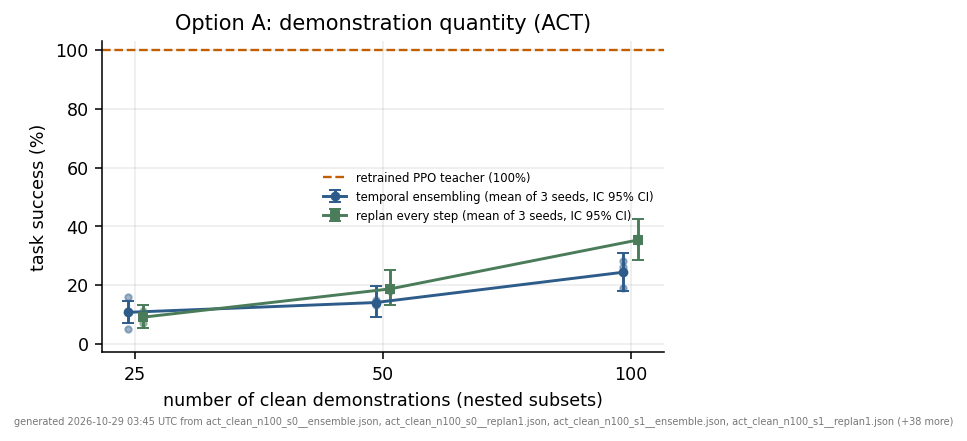
\includegraphics[width=0.49\linewidth]{figures/quantity.png}\hfill
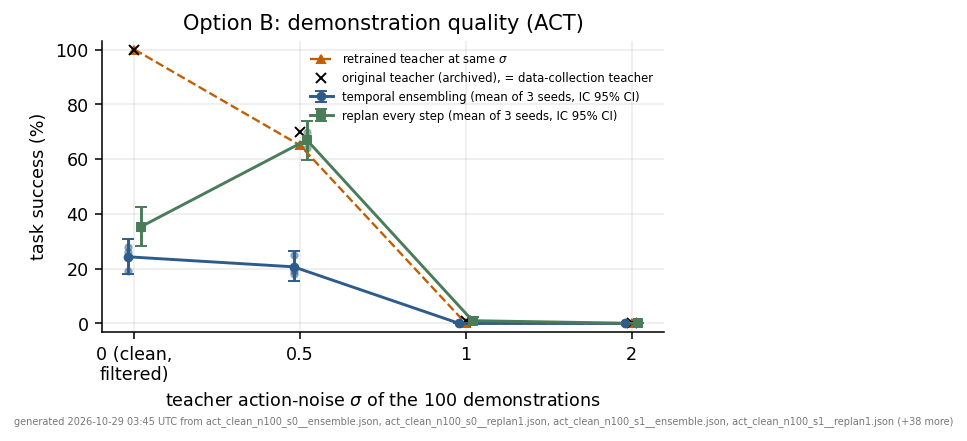
\includegraphics[width=0.49\linewidth]{figures/noise.png}
\caption{Option A (left) and Option B (right). Lines: mean of three seeds with IC
95\% intervals; dots: individual seeds; both inference modes. Right: teacher
success at each $\sigma$ (retrained teacher, dashed; original teacher, crosses).}
\label{fig:quantity}
\end{figure}

\textbf{Fresh-initialization confirmation (suite B).} Because the $\sigma=0.5$
result was first seen on the same 100 ICs used throughout, we froze a
confirmation protocol (\texttt{configs/fresh\_protocol.json}, committed and pushed
on \freshFrozen{} before any evaluation): the six existing checkpoints (clean and
$\sigma=0.5$, seeds 0--2), replanning, 100 fresh ICs from
\texttt{PRNGKey(\freshBase)} (key hash \texttt{\freshSha}; no collision with any
demonstration or suite-A key, nearest IC \freshNearest\,mm away in box/target
position), a fixed analysis and the decision rule ``confirmed iff the IC 95\%
CI of the contrast lies above 0''. Result (Table~\ref{tab:fresh},
Figure~\ref{fig:fresh}): clean \freshactcleannOneZeroZeroMean\%, $\sigma=0.5$
\freshactnoiseZeroPtFivenOneZeroZeroMean\%, $\Delta=\freshDelta$\,pp (IC CI
[\freshLo, \freshHi], 2-way [\freshTwoLo, \freshTwoHi], sign-flip $p\freshP$;
per seed \freshSeedDeltaZero, \freshSeedDeltaOne, \freshSeedDeltaTwo\,pp): the
finding is \textbf{\freshVerdict} on unseen ICs. For continuity, the
majority-vote McNemar test (an IC counts as solved if $\ge2$ of 3 seeds solve it,
a different statistic from the mean difference) gives \freshMcB{} vs \freshMcC{}
discordant ICs, $p\freshMcP$. The clean baseline scores clearly lower on the fresh ICs
(\freshactcleannOneZeroZeroMean\%) than on the original ones
(\actcleannOneZeroZeroRepMean\%; the IC intervals do not overlap), while the
$\sigma=0.5$ students score the same on both
(\freshactnoiseZeroPtFivenOneZeroZeroMean\% vs \actnoiseZeroPtFivenOneZeroZeroRepMean\%):
the original 100 ICs were apparently easier than average for the clean students,
which also means the suite-A baseline numbers are somewhat optimistic. Three
training seeds limit what can be said about other seeds.

\begin{table}[t]
\centering
\scriptsize
\begin{adjustbox}{max width=\linewidth}
\begin{tabular}{lrrrrrr}
\toprule
Suite B (replan) & Seed 0 & Seed 1 & Seed 2 & Mean & IC 95\% CI & 2-way CI \\
\midrule
ACT, 100 clean (baseline) & 21/100 & 20/100 & 20/100 & \textbf{20.3} & [14.7, 26.3] & [14.0, 27.3] \\
ACT, 100 at $\sigma{=}0.5$ & 70/100 & 67/100 & 65/100 & \textbf{67.3} & [59.7, 74.7] & [58.7, 75.7] \\
\midrule
$\sigma{=}0.5$ $-$ clean & +49 & +47 & +45 & \textbf{+47.0} & [+39.0, +54.7] & [+37.7, +56.0] \\
\bottomrule
\end{tabular}
\end{adjustbox}
\caption{Suite B, the frozen confirmation: the same six checkpoints on 100 fresh initial conditions (\texttt{PRNGKey(\freshBase)}), replanning every step, 600 episodes. Last row: noisy minus clean, per seed index and for the mean (percentage points); sign-flip $p\freshP$.}
\label{tab:fresh}
\end{table}


\begin{figure}[t]
\centering
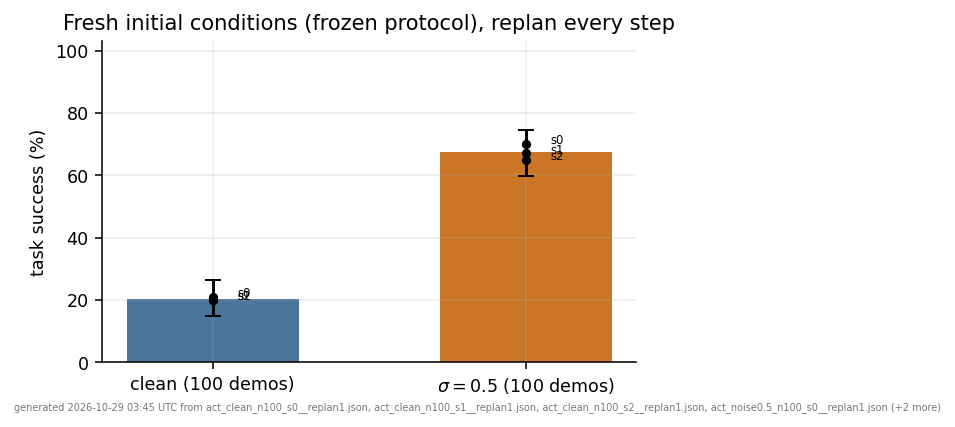
\includegraphics[width=0.5\linewidth]{figures/fresh.png}\hfill
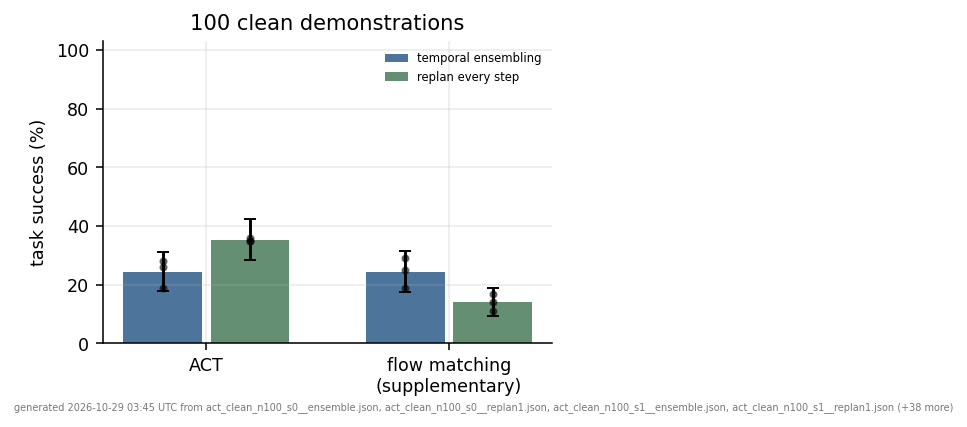
\includegraphics[width=0.45\linewidth]{figures/algorithms.png}
\caption{Left: suite B, the frozen fresh-IC confirmation (bars: mean, IC 95\%
CI; dots: seeds). Right: supplementary flow-matching arm versus ACT.}
\label{fig:fresh}
\end{figure}

\textbf{What the noise result does and does not show.} Moderate noise changes
two things at once: the actions are worse (the teacher at $\sigma=0.5$ fails
about a third of the time) and the visited states are more varied (perturbed
trajectories, including recoveries from perturbations). We did not run an
experiment that separates the two, e.g.\ noisy collection keeping only successful
episodes, or noise injected during collection but the clean action stored as the
label (DART-style). The result is consistent with the covariate-shift account in
Section~\ref{sec:fail}, but that is a hypothesis, not an isolated mechanism.

\textbf{Supplementary: flow matching.} A flow-matching policy (DiT/adaLN-Zero
denoiser over the action chunk, \nParamsFlow\,M parameters) on the same 100 clean
demos ties ACT under ensembling (\flowcleannOneZeroZeroEnsMean\% vs
\actcleannOneZeroZeroEnsMean\%) and is worse when replanning
(\flowcleannOneZeroZeroRepMean\%, \cmpActFlowRepDelta\,pp), plausibly because
resampling a fresh stochastic chunk every step makes consecutive actions
inconsistent. This arm is supplementary; the required baseline and both
ablations use ACT only.

\textbf{Historical versus corrected results.} Table~\ref{tab:oldnew} compares the
original submission's numbers (protocol v1, original checkpoints) with this
revision (v2, retrained checkpoints). The two differ by a few points per
condition, and the conclusions are unchanged. Because the checkpoints differ,
those differences are not attributable to the evaluation fix. What \emph{is}
attributable to it is measured directly: re-scoring the new rollouts with the v1
rule changes zero outcomes in all 42 evaluations, because terminated episodes
had never re-entered the success region after termination.

\begin{table}[t]
\centering
\scriptsize
\begin{adjustbox}{max width=\linewidth}
\begin{tabular}{lrrrrrr}
\toprule
Condition & v1 (orig.) & v2 (new) & flips & v1 (orig.) & v2 (new) & flips \\
\midrule
ACT, 25 clean & 11.3 & 10.7 & 0 & 7.7 & 9.0 & 0 \\
ACT, 50 clean & 14.7 & 14.0 & 0 & 19.3 & 18.7 & 0 \\
ACT, 100 clean (baseline) & 26.0 & 24.3 & 0 & 32.0 & 35.3 & 0 \\
ACT, 100 at $\sigma{=}0.5$ & 20.7 & 20.7 & 0 & 66.7 & 67.0 & 0 \\
ACT, 100 at $\sigma{=}1$ & 0.0 & 0.0 & 0 & 1.0 & 1.0 & 0 \\
ACT, 100 at $\sigma{=}2$ & 0.0 & 0.0 & 0 & 0.0 & 0.0 & 0 \\
Flow matching, 100 clean (suppl.) & 22.0 & 24.3 & 0 & 12.0 & 14.0 & 0 \\
\bottomrule
\end{tabular}
\end{adjustbox}
\caption{Historical (protocol v1, original checkpoints) versus corrected (v2, retrained checkpoints) mean success (\%), ensembling then replanning. The checkpoints differ, so the difference is NOT attributable to the evaluation fix alone. `flips' counts, on the new rollouts, the episodes (of 300) whose outcome changes between the v1 and v2 rules -- the part that IS due to the fix.}
\label{tab:oldnew}
\end{table}


\section{Failure analysis}
\label{sec:fail}
\textbf{Correcting the original analysis.} The original analysis of the baseline
(seed 0, ensembling) reported \histSucc{} successes but labelled only
\histLabelled{} episodes ``success'' and \histNever{} ``never reached the box'',
with only \histReached{} episodes inside the 12\,mm \texttt{reached\_box}
radius. Its classifier tested termination and the 12\,mm threshold
\emph{before} success, so \histMislabelled{} successful episodes received
failure labels. The 12\,mm gripper-site-to-box-centre distance is also not
evidence of reaching: among all \valN{} successful episodes in this revision
(teacher and students), every one shows finger--box contact and lifts the box by
at least \valMinLiftCm\,cm, yet only \valTwelve\% come within 12\,mm (median
closest approach \valGripMedMm\,mm, maximum \valGripMaxMm\,mm).

\textbf{Taxonomy.} Each episode now receives exactly one label, decided in a
fixed order on valid states only: success; terminated early; never touched the
box (no finger-pad/box contact in MJX's contact list); touched but never lifted
it (box never $\ge2$\,cm above its resting height); lifted but never within 5\,cm
of the target; within 5\,cm but held $<10$ steps. The thresholds were checked
against teacher and student trajectories as above and against the videos.
Counts sum to the number of failures (Table~\ref{tab:taxonomy},
Figure~\ref{fig:failure}). For the baseline with ensembling, the
\taxactcleannOneZeroZeroEnsFail{} failures are: never touched
\taxactcleannOneZeroZeroEnsNoTouch, touched but not lifted
\taxactcleannOneZeroZeroEnsNoLift, lifted but never near the target
\taxactcleannOneZeroZeroEnsLiftedFar, too short a hold
\taxactcleannOneZeroZeroEnsShortHold{} and terminated
\taxactcleannOneZeroZeroEnsTerm. So the student fails at every stage: it often
does not get the fingers onto the box, often does not achieve a grasp that
lifts it, and sometimes lifts it but does not carry it to the target. The
$\sigma=0.5$ students with replanning almost never miss the box
(\taxactnoiseZeroPtFivenOneZeroZeroRepNoTouch{} of 300) and fail mainly after
contact (\taxactnoiseZeroPtFivenOneZeroZeroRepNoLift{} not lifted,
\taxactnoiseZeroPtFivenOneZeroZeroRepLiftedFar{} lifted but far).

\begin{table}[t]
\centering
\scriptsize
%
\begin{tabular}{llrrrrrr}
\toprule
Model & Mode & Succ. & Term. & No touch & No lift & Lifted, far & Short hold \\
\midrule
ACT, 100 clean (baseline) & temporal ensembling & 73 & 6 & 82 & 91 & 28 & 20 \\
ACT, 100 clean (baseline) & replan every step & 106 & 12 & 50 & 77 & 46 & 9 \\
ACT, 100 at $\sigma{=}0.5$ & temporal ensembling & 62 & 11 & 11 & 99 & 100 & 17 \\
ACT, 100 at $\sigma{=}0.5$ & replan every step & 201 & 3 & 3 & 42 & 50 & 1 \\
\bottomrule
\end{tabular}
%
\caption{Mutually exclusive episode outcomes, pooled over 3 seeds $\times$ 100 ICs (suite A). Decision order: success; terminated early; never touched the box (no finger-pad contact); touched but never lifted it $\geq$2\,cm; lifted but never within 5\,cm of the target; within 5\,cm but held $<$10 steps.}
\label{tab:taxonomy}
\end{table}


\begin{figure}[t]
\centering
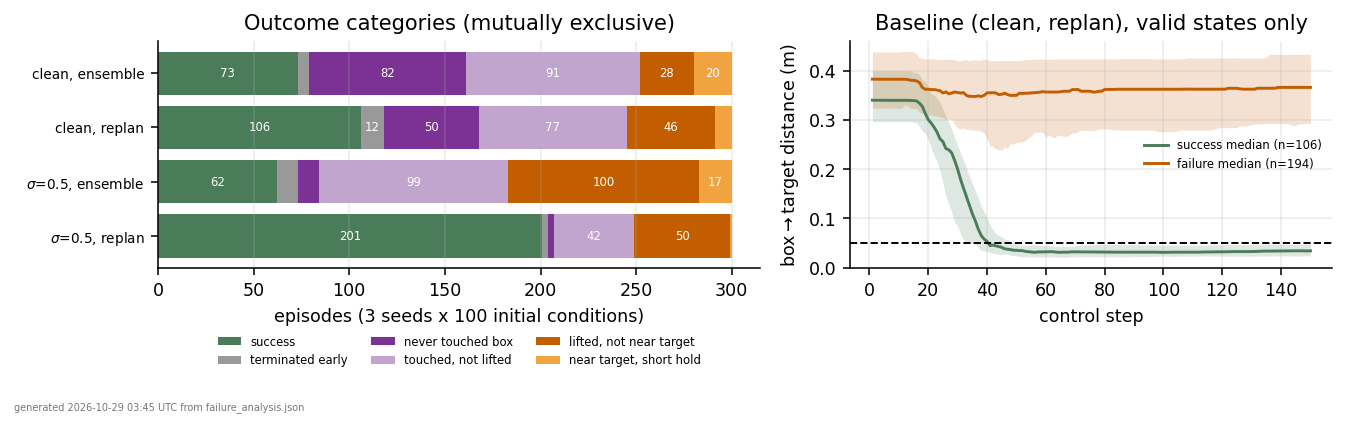
\includegraphics[width=\linewidth]{figures/failure.png}
\caption{Left: outcome categories, pooled over three seeds $\times$ 100 ICs.
Right: box--target distance of the baseline (replanning) over valid states,
median and interquartile band, by outcome.}
\label{fig:failure}
\end{figure}

\textbf{Diagnostics (separate runs, Table~\ref{tab:diag}).} (i) The student
fits its data: the one-step action error on the stored training states is
\diagMaeTrainZero--\diagMaeTrainTwo{} across seeds (action units; actions lie in
$[-1,1]$). (ii) Evaluated against the retrained teacher, the error is
\diagMaeTeacherZero{} on states the teacher visits and \diagMaeStudentZero{} on
states the student visits, about \diagMaeRatioZero$\times$ larger. The reference
here is the retrained teacher, which itself differs from the stored actions by
\diagTeacherFloor{} on the training states, so only the comparison between the
two state distributions is meaningful, not the absolute values. A low average
error on teacher states also does not rule out small, control-sensitive errors
at critical moments such as closing the gripper. (iii) The student is only
slightly better on the ICs its demonstrations came from than on held-out ICs
(ensembling \diagTrainEnsZero/\diagTestEnsZero,
\diagTrainEnsOne/\diagTestEnsOne, \diagTrainEnsTwo/\diagTestEnsTwo{} successes per
seed), so the gap to the teacher is not a matter of unseen initial
conditions. (iv) Inference: executing whole chunks open loop is worst;
ACT-reference ensemble weighting (oldest prediction weighted most) is no better
than the historical weighting; replanning is best.

\begin{table*}[t]
\centering
\scriptsize
\resizebox{\linewidth}{!}{%
\begin{tabular}{lrrrrrrrr}
\toprule
Baseline & Ens.\ train/test & Replan train/test & MAE data & MAE teacher & MAE student & Ens.\ (ACT order) & Open loop & Chunk 5 \\
\midrule
seed 0 & 38 / 27 & 38 / 35 & 0.031 & 0.073 & 0.653 & 26 & 10 & 25 \\
seed 1 & 32 / 21 & 35 / 34 & 0.031 & 0.073 & 0.651 & 18 & 6 & 25 \\
seed 2 & 27 / 28 & 33 / 31 & 0.032 & 0.075 & 0.662 & 28 & 9 & 23 \\
\bottomrule
\end{tabular}
}
\caption{Separate diagnostic runs on the three baseline models (ACT, 100 clean). Columns 2--3: successes out of 100 on the ICs the demonstrations came from vs.\ the held-out ICs. MAE: mean absolute error of the first predicted action on the stored training states (vs.\ stored actions) and on states visited by the retrained teacher or by the student (vs.\ the retrained teacher; its own disagreement with the stored actions on training states is \diagTeacherFloor). Last three: successes of other inference variants.}
\label{tab:diag}
\end{table*}


\textbf{Interpretation.} Together these point to compounding error under
covariate shift, the standard behaviour-cloning failure: the policy is accurate
where the teacher goes and drifts into states the demonstrations do not cover,
where nothing teaches it to recover. Replanning every step limits how long an
error persists, and noisy demonstrations add perturbed and recovering states to
the data, which fits both of our main effects. This is the best-supported
explanation, not a proven one: the diagnostics show the error grows off the
teacher's distribution, not that coverage is the only cause, and the noise
ablation does not separate coverage from action quality.

\textbf{Determinism and the videos.} Batched GPU evaluation is not
bit-reproducible: re-running the same 100-episode evaluation reproduces
\videoAgreeMin--\videoAgreeMax{} of the 100 outcomes, so per-model success rates
are reproducible to within a few episodes (the diagnostic re-runs in
Table~\ref{tab:diag} show the same effect). The videos are therefore never named
after a different run. Each clip comes from one batched 100-episode rollout,
is labelled by that rollout's own outcome, and is accepted only if re-scoring
the rendered states reproduces the label exactly.

\section{Reproducibility and reflection}
\textbf{Software.} Python \verpython, jax/jaxlib \verjax{} (CUDA\,12), flax
\verflax, brax \verbrax, mujoco and mujoco-mjx \vermujoco,
\texttt{playground} \verplayground{} at commit \texttt{\playgroundSha} (assets:
mujoco\_menagerie \texttt{\menagerieSha}), torch \vertorch, numpy \vernumpy.
Hardware: \gpuName{}. Full pins: \texttt{configs/requirements.lock.txt}.

\textbf{Commands.} \texttt{README.md} lists every step:
\texttt{setup\_env.sh}; \texttt{stage1r\_teacher.py} (teacher, teacher evaluation,
dataset audit); \texttt{stage2\_train.py} (21 models); \texttt{stage2\_eval.py
-{}-suite A/B}; \texttt{stage2b\_failure.py}, \texttt{diag\_student.py},
\texttt{diag\_replay.py}; \texttt{collect\_run\_artifacts.py};
\texttt{stage3\_report.py} (CPU only, builds this PDF from committed results);
\texttt{package.py}. Paths derive from the checkout. Training and evaluation
resume only when a stored identity (dataset, configuration, code, checkpoint and
evaluation-key hashes, protocol version) matches. Checkpoints are attached to the
repository as release assets with SHA-256 hashes
(\texttt{results/checkpoints\_manifest.json}). Seeds: students $\{0,1,2\}$;
suite A \texttt{split(PRNGKey(7777),100)}; suite B
\texttt{split(PRNGKey(\freshBase),100)}; demonstrations
\texttt{split(PRNGKey(1000+$\lfloor1000\sigma\rfloor$),512)}; PPO seed 0.

\textbf{Environment issues worth recording.} (i) Our GPU nodes have no NVIDIA
graphics userspace, so the assignment's EGL snippet cannot run there; videos are
rendered with software OSMesa from a side conda prefix
(\texttt{HW2\_GL=osmesa}), configured before \texttt{mujoco} is imported because
PyOpenGL resolves \texttt{libOSMesa} via \texttt{ctypes.util.find\_library}, which
ignores \texttt{LD\_LIBRARY\_PATH}. (ii) brax 0.14.2 calls
\texttt{jax.device\_put\_replicated}, removed in newer jax, hence the jax/flax
pins. (iii) MJX reproduces an initial condition exactly (stored versus re-reset
observations agree to \replayResetDev), but replaying a stored action sequence
diverges chaotically at floating-point level (deviation $>10^{-3}$ first at steps
\replayFirstBig{} in three episodes), because batched and single-environment
rollouts do not run identical kernels. Videos are therefore rendered from the
\emph{same} batched rollout that is scored, not from a single-environment replay.

\textbf{Runtime (measured).} Teacher: \teacherWallMin{} minutes of PPO on one
A100. Students: \trainMinAct{} minutes per ACT model and \trainMinFlow{} per flow
model, eight at a time on four A100s (about 15 minutes for all 21). Evaluation:
about \evalSecMean{}\,s per model, mode and 100 ICs. The CPU-only report rebuild
takes about a minute plus LaTeX.

\textbf{Limitations.} Three training seeds per condition; one task; one success
definition (5\,cm, 10 steps); a retrained teacher that is not the
data-collecting teacher, so teacher-referenced diagnostics are approximate;
evaluation reproducible only to within a few episodes per model; and the noise
ablation confounds action quality with state coverage.

\textbf{With more data, compute or time.} (i) Separate coverage from quality:
inject noise during collection but store the clean teacher action (DART), and
collect noisy data keeping only successful episodes. (ii) Attack covariate shift
directly with DAgger-style relabelling by the teacher. (iii) More training seeds
and a deterministic evaluation mode (deterministic XLA/cuDNN kernels), so
per-model numbers reproduce exactly. (iv) Check the conclusions on a second
manipulation task and under other success radii.

\begin{table}[t]
\centering
\scriptsize
\begin{tabular}{p{0.30\linewidth}p{0.62\linewidth}}
\toprule
Artifact & Produced from \\
\midrule
\texttt{results/figures/ppo\_curve.png} & \texttt{runs/teacher/ppo\_progress.json} \\
\texttt{results/figures/demos.png} & \texttt{data/demos\_sigma0.npz} \\
\texttt{results/figures/demo\_frames.png} & \texttt{videos/expert\_demo*\_frames.npz} \\
\texttt{results/figures/loss.png} & \texttt{runs/conditions/*/train\_log.json} \\
\texttt{results/figures/quantity.png} & \texttt{results/conditions/*.json} \\
\texttt{results/figures/noise.png} & \texttt{results/conditions/*.json} \\
\texttt{results/figures/algorithms.png} & \texttt{results/conditions/*.json} \\
\texttt{results/figures/failure.png} & \texttt{results/failure\_analysis.json} \\
\texttt{results/tables/main.tex} & \texttt{results/conditions/*.json} \\
\texttt{results/tables/data.tex} & \texttt{runs/teacher/stage1\_report.json} \\
\texttt{results/tables/paired.tex} & \texttt{results/paired\_comparisons.json} \\
\texttt{results/tables/modes.tex} & \texttt{results/conditions/*.json} \\
\texttt{results/summary.csv} & \texttt{results/conditions/*.json} \\
\bottomrule
\end{tabular}
\caption{Provenance of every figure and table in this report.}
\label{tab:prov}
\end{table}


\section{Citations and use of tools}
\begin{itemize}
\item MuJoCo Playground: Zakka et al., \emph{MuJoCo Playground}, 2025,
\url{https://arxiv.org/abs/2502.08844}; code
\url{https://github.com/google-deepmind/mujoco_playground} (commit
\texttt{\playgroundSha}). Environment, PPO hyperparameters and the random-action
snippet of the assignment.
\item MuJoCo Menagerie (Panda model): \url{https://github.com/google-deepmind/mujoco_menagerie}.
\item ACT: Zhao et al., \emph{Learning Fine-Grained Bimanual Manipulation with
Low-Cost Hardware}, RSS 2023, \url{https://arxiv.org/abs/2304.13705}; reference
implementation \url{https://github.com/tonyzhaozh/act}. Re-implemented with the
deviations of Section~3.
\item Diffusion Policy (the alternative the assignment names; not used): Chi et
al., RSS 2023, \url{https://arxiv.org/abs/2303.04137}.
\item Flow matching (supplementary arm): Lipman et al., ICLR 2023,
\url{https://arxiv.org/abs/2210.02747}; Liu et al., ICLR 2023,
\url{https://arxiv.org/abs/2209.03003}; DiT/adaLN-Zero: Peebles and Xie, ICCV
2023, \url{https://arxiv.org/abs/2212.09748}.
\item Brax (PPO): Freeman et al., \url{https://github.com/google/brax}.
\item Covariate shift in behaviour cloning: Ross, Gordon and Bagnell, \emph{A
Reduction of Imitation Learning and Structured Prediction to No-Regret Online
Learning} (DAgger), AISTATS 2011; noise injection during demonstration: Laskey
et al., \emph{DART}, CoRL 2017, \url{https://arxiv.org/abs/1703.09327}.
\item \textbf{LLM use.} An LLM coding assistant (Anthropic's Claude, in Claude
Code) wrote and debugged most of the implementation, the cluster job scripts
and the evaluation and statistics code, diagnosed the OSMesa and jax/brax
environment problems, and drafted this report, in both the original submission
and this revision. In the revision it also audited the original code, found the
termination and failure-labelling errors described in Section~\ref{sec:fail},
implemented the fixes and tests, retrained and re-evaluated all models, and
rewrote the report. Every number in this report is generated by
\texttt{stage3\_report.py} from stored result files (each quantity in the prose
is a LaTeX macro, not typed by hand). The author specified the assignment
scope and the revision requirements and is responsible for the submission.
\end{itemize}

\end{document}
